\chapter{Chess-game analysis}

\section{The game of chess}

Chess is a two-player strategy board game played on a checkered board with 64 squares arranged in an 8×8 grid.

The history of chess was firstly documented around 6th Century, although the earliest origins are ambiguous. It is believed that the game's predecessor was originated in India, from where the game spread to Persia. After the Arabic occupation, the game was spread through the Muslim world and to Southern Europe, where it evolved into the current form in the 15th Century ~\cite{murray1913history}.


    \begin{figure}[H]
        \centering
        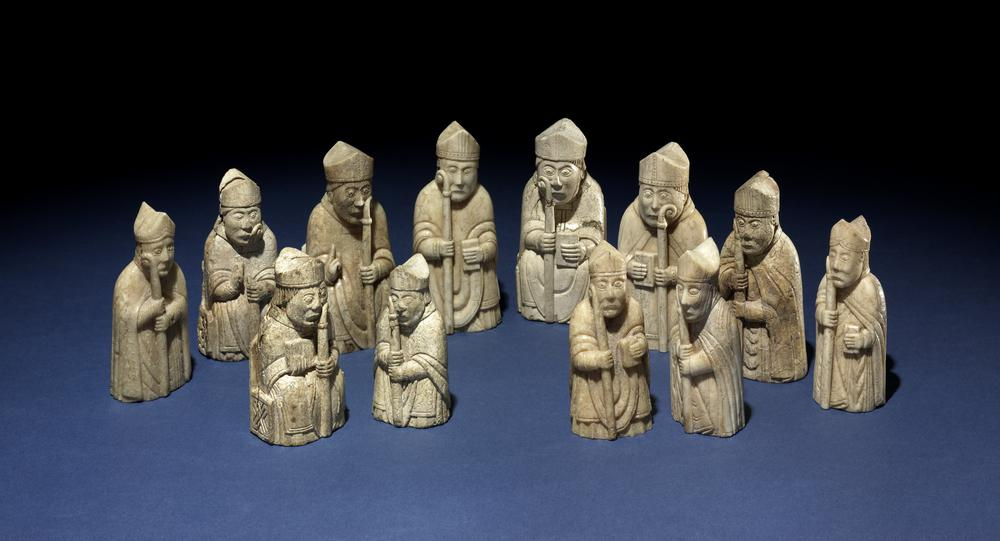
\includegraphics[width=0.5\textwidth]{chessmen}
        \caption{The Lewis chessmen are a group of distinctive 12th-century chess pieces, along with other game pieces, most of which are carved from walrus ivory. Present location: British Museum, London. Image courtesy of Wikipedia Commons}.
    \end{figure}

\section{Computing chess}
